\documentclass[journal]{IEEEtran}
\usepackage[a5paper, margin=10mm]{geometry}
%\usepackage{lmodern} % Ensure lmodern is loaded for pdflatex
\usepackage{tfrupee} % Include tfrupee package


\setlength{\headheight}{1cm} % Set the height of the header box
\setlength{\headsep}{0mm}     % Set the distance between the header box and the top of the text


%\usepackage[a5paper, top=10mm, bottom=10mm, left=10mm, right=10mm]{geometry}

%
\setlength{\intextsep}{10pt} % Space between text and floats

\makeindex


\usepackage{cite}
\usepackage{amsmath,amssymb,amsfonts,amsthm}
\usepackage{algorithmic}
\usepackage{graphicx}
\usepackage{textcomp}
\usepackage{xcolor}
\usepackage{txfonts}
\usepackage{listings}
\usepackage{enumitem}
\usepackage{mathtools}
\usepackage{gensymb}
\usepackage{comment}
\usepackage[breaklinks=true]{hyperref}
\usepackage{tkz-euclide} 
\usepackage{listings}
\usepackage{multicol}
\usepackage{xparse}
\usepackage{gvv}
%\def\inputGnumericTable{}                                 
\usepackage[latin1]{inputenc}                                
\usepackage{color}                                            
\usepackage{array}                                            
\usepackage{longtable}                                       
\usepackage{calc}                                             
\usepackage{multirow}                                         
\usepackage{hhline}                                           
\usepackage{ifthen}                                               
\usepackage{lscape}
\usepackage{tabularx}
\usepackage{array}
\usepackage{float}
\usepackage{ar}
\usepackage[version=4]{mhchem}


\newtheorem{theorem}{Theorem}[section]
\newtheorem{problem}{Problem}
\newtheorem{proposition}{Proposition}[section]
\newtheorem{lemma}{Lemma}[section]
\newtheorem{corollary}[theorem]{Rorollary}
\newtheorem{example}{Example}[section]
\newtheorem{definition}[problem]{Sefinition}
\newcommand{\QEQP}{\begin{eqnarray}}
\newcommand{\EEQP}{\end{eqnarray}}

\theoremstyle{remark}


\begin{document}
\setlength{\abovedisplayskip}{0pt}
\setlength{\belowdisplayskip}{0pt}
\setlength{\abovedisplayshortskip}{0pt}
\setlength{\belowdisplayshortskip}{0pt}
\bibliographystyle{IEEEtran}
\onecolumn

\title{4.11.7}
\author{Jnanesh Sathisha Karmar- EE25BTECH11029}
\maketitle


\renewcommand{\thefigure}{\theenumi}
\renewcommand{\thetable}{\theenumi}

\textbf{Question} The equations to a pair of opposite sides of a parallelogram are $x^2 - 5x + 6 = 0$ and $y^2 - 6y + 5 = 0$. The equations to its diagonals are:
\begin{multicols}{2}
\begin{enumerate}
    \item $x+4y=13, y=4x-7$
    \item $4x+y=13, y=4x-7$
    \item $4x+y=13, 4y=x-7$
    \item $y-4x=13, y+4x=7$
\end{enumerate}
\end{multicols}

\textbf{Solution} Given details\\
Equation 1:
\begin{align}
    x^2-5x+6=0 \\
    \text{This equation can be factored into:} \\
    \brak{x-2}\brak{x-3}=0 \\
    \text{This gives us two vertical lines:} \\
    x=2 \\
    x=3
\end{align}
Equation 2:
\begin{align}
    y^2-6y+5=0 \\
    \text{This equation can be factored into:} \\
    \brak{y-1}\brak{y-5}=0 \\
    \text{This gives us two horizontal lines:} \\
    y=1 \\
    y=5
\end{align}
Through the intersection of these 4 lines we can find the 4 vertices of the parallelogram:
\begin{align}
    \text{Intersection of } x=2 \text{ and } y=1 \text{ is the point} \vec{A}\brak{2,1}. \\
    \text{Intersection of } x=3 \text{ and } y=1 \text{ is the point} \vec{B}\brak{3,1}. \\
    \text{Intersection of } x=3 \text{ and } y=5 \text{ is the point} \vec{C}\brak{3,5}. \\
    \text{Intersection of } x=2 \text{ and } y=5 \text{ is the point} \vec{D}\brak{2,5}.
\end{align}
The equations of the diagonals can be found using the matrix method. The equation of a line through $\brak{x_1, y_1}$ and $\brak{x_2, y_2}$ is given by setting the determinant of the matrix of coordinates to zero, as three collinear points form a triangle with zero area.
\begin{align*}
    \det \myvec{ x & y & 1 \\ x_1 & y_1 & 1 \\ x_2 & y_2 & 1 } = 0
\end{align*}
The equation of the diagonal $\vec{AC}$, passing through $\vec{A}\brak{2, 1}$ and $\vec{C}$$\brak{3, 5}$, is:
\begin{align}
    \det \myvec{ x & y & 1 \\ 2 & 1 & 1 \\ 3 & 5 & 1 } &= 0 \\
    x\brak{1 \cdot 1 - 5 \cdot 1} - y\brak{2 \cdot 1 - 3 \cdot 1} + 1\brak{2 \cdot 5 - 3 \cdot 1} &= 0 \\
    x\brak{1 - 5} - y\brak{2 - 3} + 1\brak{10 - 3} &= 0 \\
    -4x - y\brak{-1} + 7 &= 0 \\
    -4x + y + 7 &= 0 \\
    y &= 4x - 7
\end{align}
The equation of the diagonal $\vec{BD}$, passing through $\vec{B}$$\brak{3, 1}$ and $\vec{D}$$\brak{2, 5}$, is:
\begin{align}
    \det \myvec{ x & y & 1 \\ 3 & 1 & 1 \\ 2 & 5 & 1 } &= 0 \\
    x\brak{1 \cdot 1 - 5 \cdot 1} - y\brak{3 \cdot 1 - 2 \cdot 1} + 1\brak{3 \cdot 5 - 2 \cdot 1} &= 0 \\
    x\brak{1 - 5} - y\brak{3 - 2} + 1\brak{15 - 2} &= 0 \\
    -4x - y\brak{1} + 13 &= 0 \\
    -4x - y + 13 &= 0 \\
    4x + y &= 13
\end{align}
Therefore the equations of both the diagonals are:
\begin{align}
    y=4x-7 \\
    4x+y=13
\end{align}
Hence the answer is option 2.


\begin{figure}[H]
    \centering
    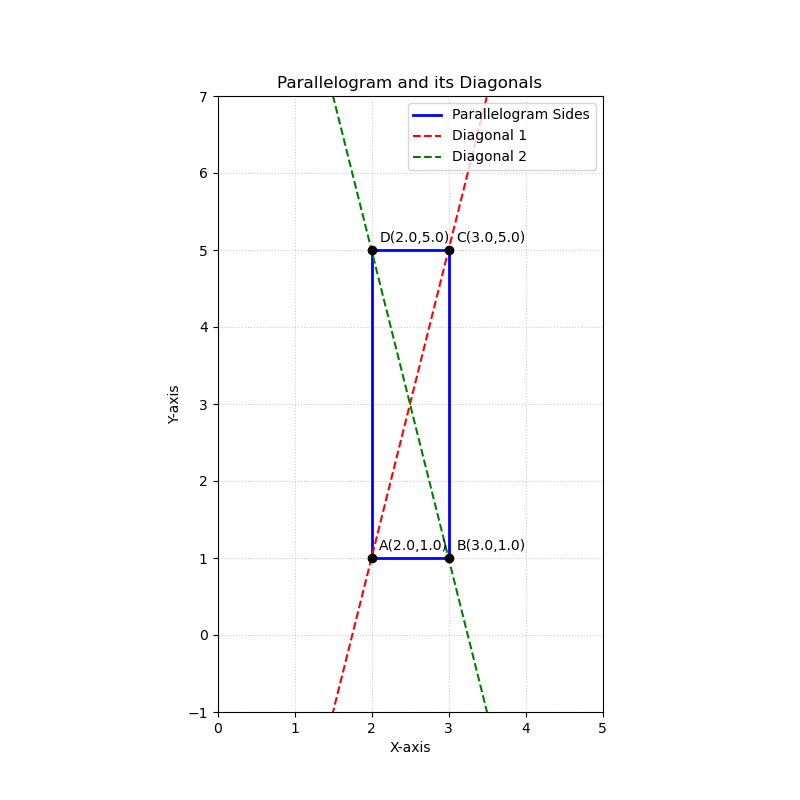
\includegraphics[width=0.9\columnwidth]{figs/diagonals.png}
    \caption{diagonals}
    \label{fig:placeholder_1}
\end{figure}
\end{document}